\section{$Re_{\tau}=1000$ simulation} 
The second simulation performed is carried out at $Re_{\tau}=1000$, which in terms of channel width and bulk velocity is equivalent to $Re_{b}\approx40000$.\par
The bulk velocity, obtained as shown in~\ref{bulk:velocity}, is 19.99, while $\alpha_{0}$ and $\beta_{0}$ are respectively 0.5 and 1, in order to reproduce the correct dimensions of the channel, as shown in chapter~\ref{chapter:Re180}.\par
Since the high computational cost needed to obtain these results we were unable to carry out a complete simulation. Thus the results reported shows the statistics associated with a flow in transitory phase. \\~\par

The simulation employed a variable timestep, determined through the Courant-Friedrichs-Lewy condition.
The CFL limit has been set to 1.6, close to the theoretical ones, equal to $\sqrt{3}$, for a third-order Runge-Kutta method. Such choice has been influenced by the high computational cost needed to compute the CFL. In fact, carry out such value requires three different transpositions and relative Fourier transformations. Therefore we decided to perform such computation approximately on every 10 steps. In this way the gain in terms of performance is significant, combining the flexibility of the Courant-Friedrichs-Lewy condition with a reduced cost to compute it.\par

The grid employed in this simulation face 500 points in the wall-normal direction, 2048 in the spanwise direction and 2048 points along the streamwise dimension, direction in which we exploit the Hermitian symmetry. According to this configuration, the grid size reach the billion of points.\par
Table~\ref{table:1000} report a summary of the simulation configuration for the $Re_{\tau}=1000$ case.\\~\par

\begin{table}
\caption{Simulation data for $Re_{\tau}$=1000}
\begin{center}
\begin{tabular}{ccccccccccccc}
\toprule
$L_{x}$ & $L_{z}$ & $\delta$ & $nx$ & $nz$ & $ny$ & $\alpha_{0}$ & $\beta_{0}$ & $\Delta x^{+}$ & $\Delta z^{+}$ & $px$ & $CFL$\\
$4\pi$ & $2\pi$ & 1 & 2048 & 2048 & 500 & 0.5 & 1 & 6.1  & 3 & 1 & 1.6 \\
\bottomrule
\end{tabular}
\end{center}
\label{table:1000}
\end{table}


Since are required approximately 50GB of disk space per each field we decided to avoid to save them on disk, instead we calculated the statistics runtime, merging the files at the end of the simulation, reducing the required space to few KB.\\~\par

The results that we will present shortly are obtained through the ensemble average of 100 fields, and cover 0.1 non dimensional time units. In this lapse of time the mean $Re_{\tau}$ is approximately 991 units.\par
Let us focus now on the statistics gained from the simulation.\\~\par
Figure~\ref{loglaw:1000} report the law of the wall. As we can see from the plot, made in semi-logarithmic scale using the wall units, our data fits the theoretical curve throughout the logarithmic region, while, towards the centerline, a residual sensitivity to the initial conditions is still present and lead to few differences with the results obtained by Moser \& Lee in~\cite{Lee}.\par
Far from the wall, the velocity defect law find good feedback with our results, as shown by the graph~\ref{velocity:defect:1000}.\\~\par

\begin{figure}
\begin{center}
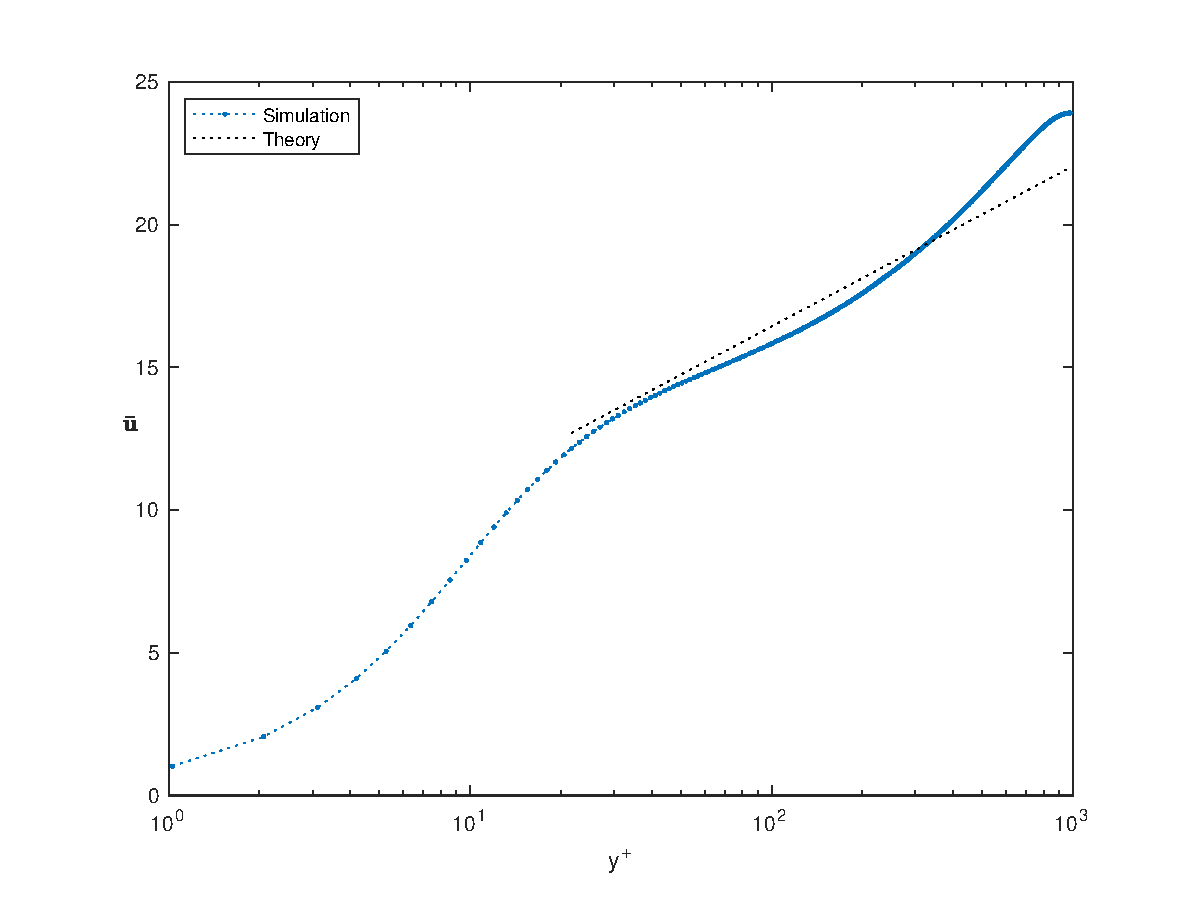
\includegraphics[scale=0.55]{grafici/loglaw_1000.eps}
\caption{$\bar{u}^{+}$ in the near wall region for a $Re_{\tau}=1000$ simulation}
\label{loglaw:1000}
\end{center} 
\end{figure}

\begin{figure}
\begin{center}
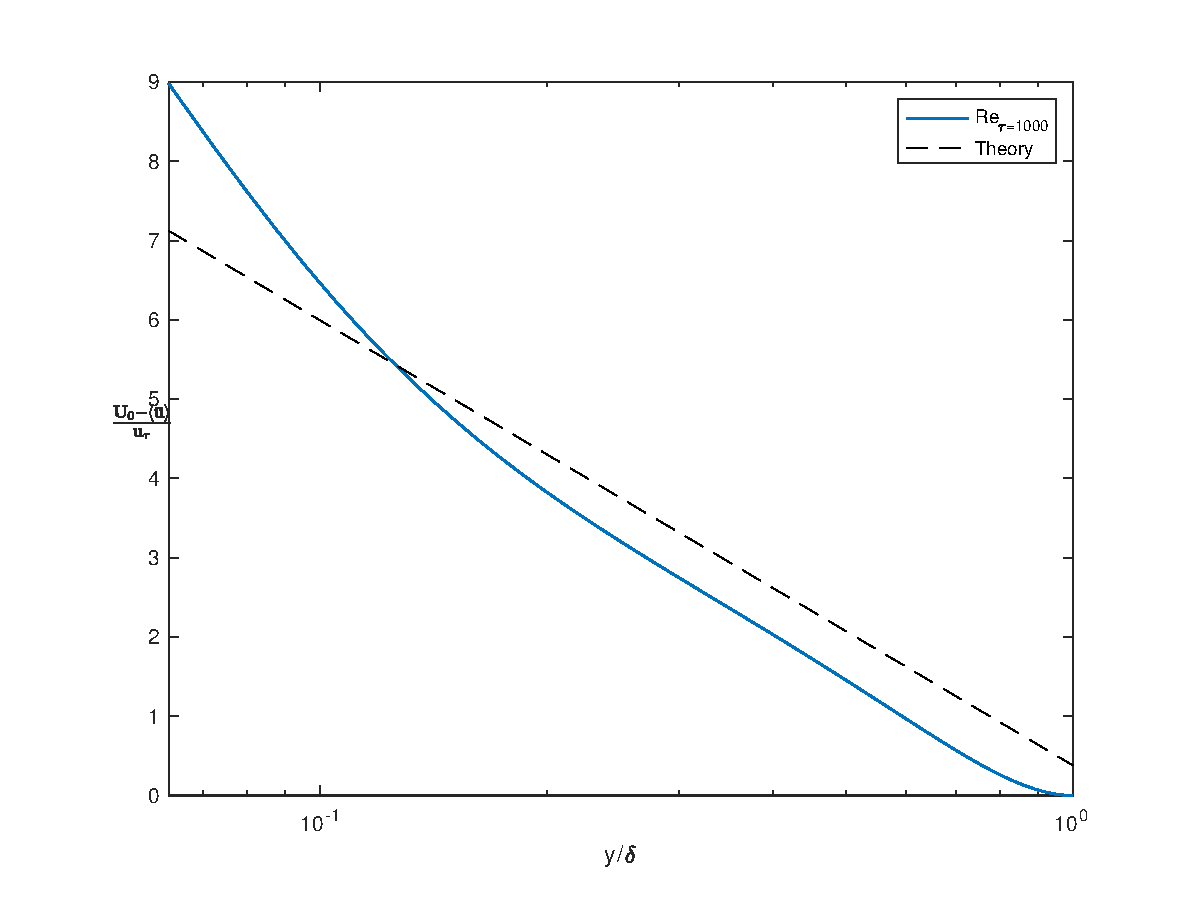
\includegraphics[scale=0.55]{grafici/velocity_defect_1000.eps}
\caption{Velocity defect for a $Re_{\tau}=1000$ simulation}
\label{velocity:defect:1000}
\end{center} 
\end{figure}

In figure~\ref{budget:1000} we reported the \emph{rms} fluctuations, normalized by the $u_{\tau}^{2}$, jointed with the TKE distribution. The first differences that we can immediately face by comparing our curves with the ones in figure~\ref{k+budgets:180} are the peak values. These values tends to increase with respect to the counterpart of the $Re_{\tau}=180$ simulation, highlighting how this simulation contains more energy than the previous ones.\par
Although there is an higher content of energy, the curves shape remains aligned with the ones seen in the previous chapter.\par
The near-wall behavior present a two-components turbulent flow. In fact, as evidenced by the magnification, the wall-normal fluctuations are absent for the first few units.
\\~\par

The production curve does not exhibit marked difference across the results of this simulation and the $Re_{\tau}=180$ simulation, as depicted in figure~\ref{tke:prod:1000}.\\~\par

\begin{figure}
\begin{center}
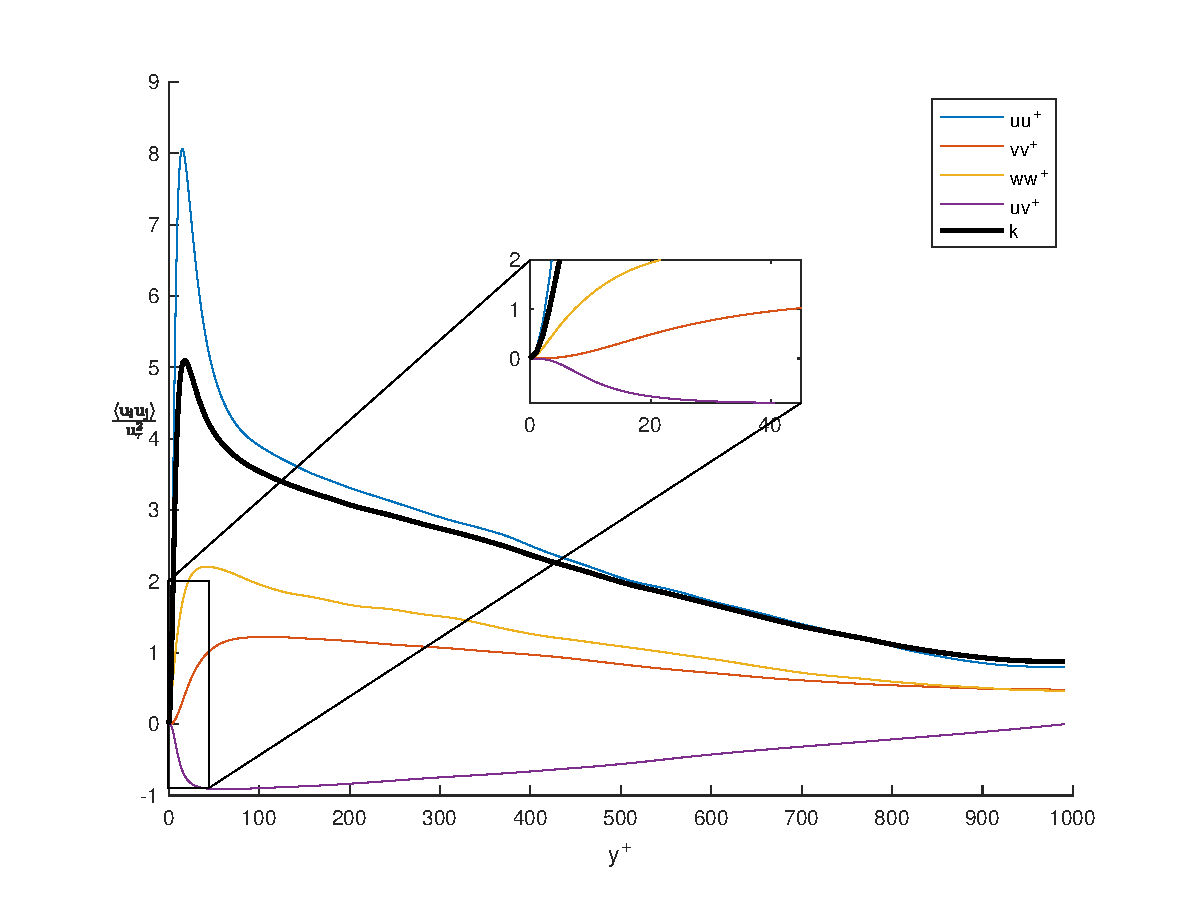
\includegraphics[scale=0.55]{grafici/budget+k_1000.eps}
\caption{\emph{rms} terms for a $Re_{\tau}=1000$ simulation}
\label{budget:1000}
\end{center} 
\end{figure}


The finer mesh and the higher Reynolds evidenced the appearance of a new turbulence peak, detached from the wall-cycle, identified by knees in the curves represented in figure~\ref{rms:1000}. Although the profiles are similar, with exception for the higher peaks reached, in the near wall region, they behave differently moving towards the inner region of the flow. In particular, by looking at $u'/u_{\tau}$, the sketchy knee present around $y^{+}\approx 100$ in figure~\ref{rms:kmm:180} now results to be fully developed and has moved towards the centerline, approximately around $y^{+}\approx 400$. The peak does not differ too much in the two simulations, with values of $2.6\sim2.7$ located at $y^{+}\approx14$, however, the higher energy content manifest through the trailing values. These terms shows an upward bias, if compared with the $Re_{\tau}=180$ values, plus the presence of the already cited knee.\par
Similar behavior is expressed by $w'/u_{\tau}$, although in its case the increase in terms of peak value is consistent, with a slightly decrease of the peak coordinate towards $y^{+}\approx30$. Also in this case the appearance of the knee is approximately around $y\approx 400$.\par
Also the term $v'/u_{\tau}$ face a huge increment of the peak value, in first approximation we may say that it doubles its value with respect to $Re_{\tau}=180$ simulation. In such case identifying the knee is less straightforward. However, we can observe that the area under the curve has clearly increased.\\~\par

\begin{figure}
\begin{center}
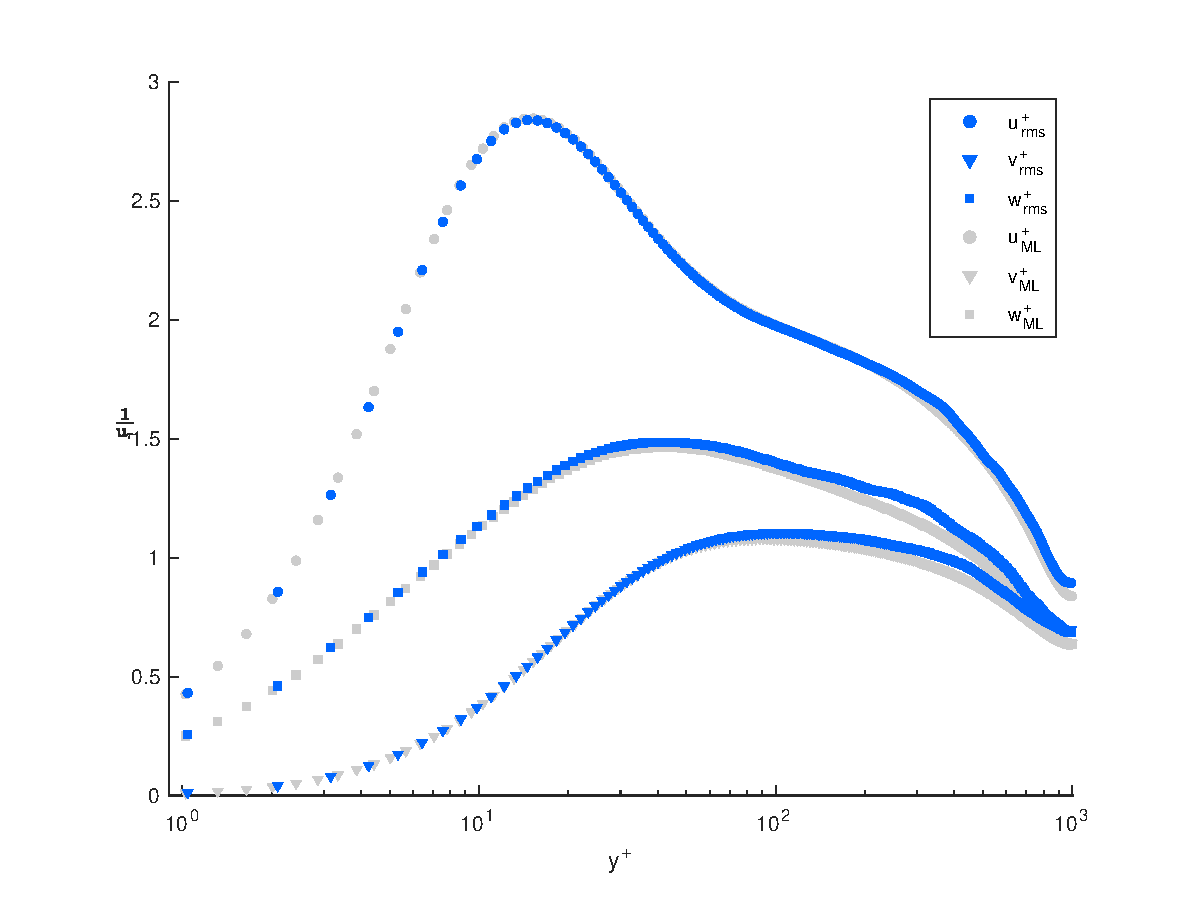
\includegraphics[scale=0.55]{grafici/rms_1000.eps}
\caption{\emph{rms} behavior on a $Re_{\tau}=1000$ simulation}
\label{rms:1000}
\end{center} 
\end{figure}

\begin{figure}
\begin{center}
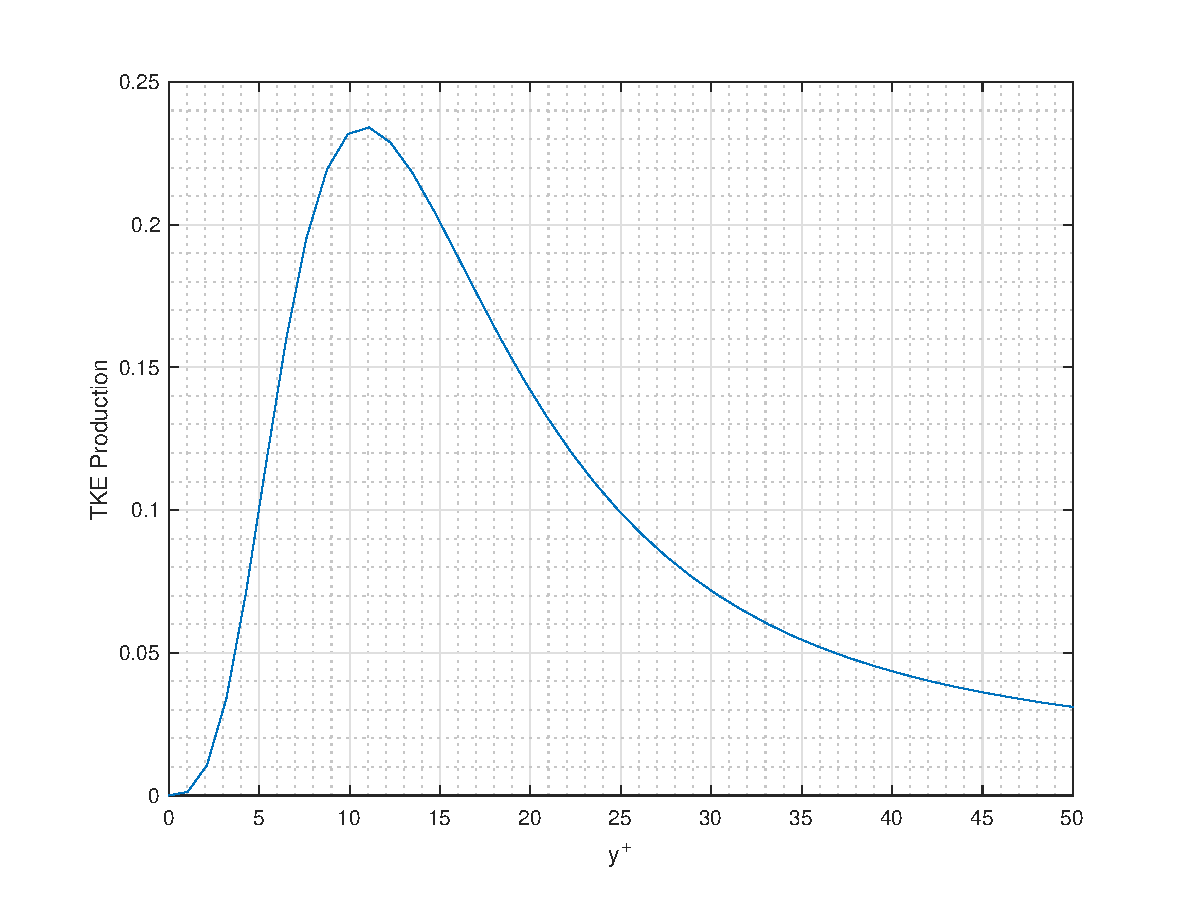
\includegraphics[scale=0.55]{grafici/tke_prod_1000.eps}
\caption{Production term of the TKE eq. for a $Re_{\tau}=1000$ simulation}
\label{tke:prod:1000}
\end{center} 
\end{figure}

An upward shift is expressed also by the \emph{rms} terms near the wall. Nevertheless the curves does not exhibit marked changes in shape with respect to its counterpart in the previous simulation, as figure~\ref{wall:rms:1000} testify, with the streamwise and spanwise components that depart from zero as $y^{+}$, while the wall-normal components leave the wall as $y^{2+}$. \\~\par

Similar reasoning applies also for the graphs of the \emph{production}, reported in figure~\ref{tke:prod:1000}, that reach a slightly higher peak of $P/Re_{\tau}=0.24$, without showing significant changes of the curve shapes. The peak is still located nearby $y\approx 12$.\\~\par

As theory affirms, the wall coordinate of the peak of production corresponds to that in which the stress components become equivalent. This aspect will be detailed further, comparing the results of all the simulations together.
At the present we limit to present the behavior of the stress components, which is reported in figure~\ref{stresses:1000}.

\begin{figure}
\begin{center}
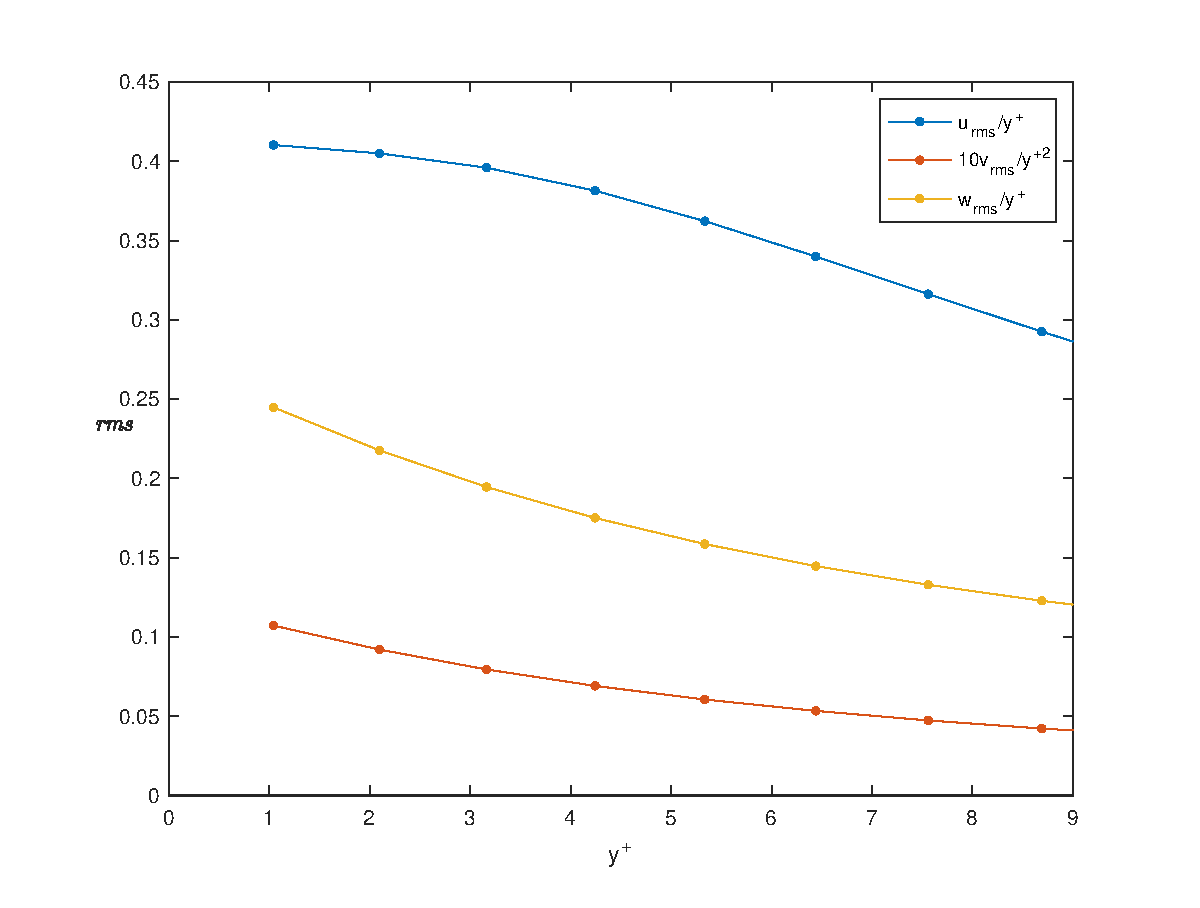
\includegraphics[scale=0.55]{grafici/wall_rms_1000.eps}
\caption{Normalized \emph{rms} close to the wall for a $Re_{\tau}=1000$ simulation}
\label{wall:rms:1000}
\end{center} 
\end{figure}

\begin{figure}
\begin{center}
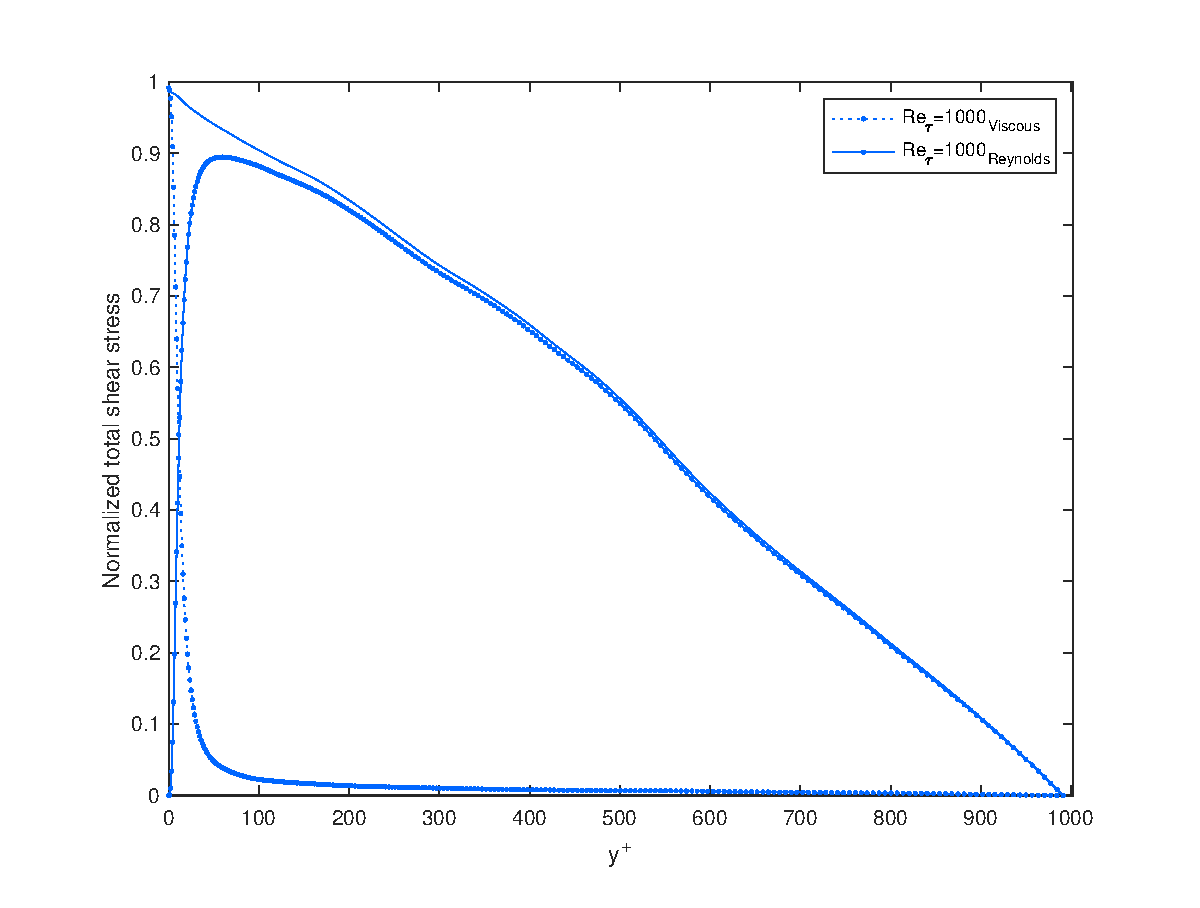
\includegraphics[scale=0.55]{grafici/stresses_1000.eps}
\caption{Normalized total shear stress for a $Re_{\tau}=1000$ simulation}
\label{stresses:1000}
\end{center} 
\end{figure}